%! Author = ashutosh
%! Date = 4/20/22

\documentclass{article}
\usepackage[letterpaper,top=2cm,bottom=2cm,left=3cm,right=3cm,marginparwidth=1.75cm]{geometry}
\usepackage[english]{babel}
\usepackage{float}
\usepackage{amsmath}
\usepackage{graphicx}
\usepackage{caption}
\usepackage{subcaption}
\usepackage[utf8]{inputenc}
\usepackage{fancyhdr}
\usepackage{listings}
\usepackage{subfig}
\usepackage[table,xcdraw,svgnames]{xcolor}
\usepackage{natbib}
\usepackage[colorlinks]{hyperref}
\AtBeginDocument{%
\hypersetup{
    colorlinks=true,
    citecolor=green,
    linkcolor=blue,
    filecolor=cyan,
    urlcolor=magenta,
    }

}
\def\at#1{{\color{red}\textbf{AT fix this: #1}}\xspace}

\title{Investigating Structure of Bias Manifold and Bias Evolution}


\author{Ashutosh Tiwari\\
	\normalsize ashutiwa@iu.edu
}

\pagestyle{fancy}
\fancyhf{}
\lhead{Presented as a project for  MGMT ACCESS USE BIG DATA(FALL 2022)}
\rfoot{Page \thepage}
\begin{document}
\maketitle



\section{Background}

Bias is an inseparable part of output models of considerable size. This bias is generally the result of data itself on which model is trained. This bias is tackled in general at three different stages in previous works. Some research (example ~\cite{DBLP:journals/corr/BolukbasiCZSK16a}) suggests that probably we should try to fix this bias after the model is trained and then debias the generated model embeddings. There is one more approach to learn models  that are fair (free from accumulated bias in dataset). This requires having two "unfair" models and then training a new model in presence of an adversercial setting ~\cite{kenna_using_2021}. However we think that all these methods are bandaid at best, because of these reasons \begin{itemize}
    \item These limit usability and scope of a dataset and set of modeling techniques that can be applied to same. Because both of these rely on first training the model, these are methods are not generic enough both to be able to train any model on the dataset.
    \item These are very inefficient in terms of computing needs because first they need to train the model and then remove bias from embeddings/model.

\end{itemize}

Therefore a third method is to rather remove biases from the dataset itself ~\cite{ravfogel_null_2020}. Keeping these points in mind, I've designed this project so that our analysis can be used to guess the structure of biases, calculate biases and provide us with tools to identify the most biased documents from the dataset. Hopefully all these available tools can then be used to remove biases from the dataset itself.


\\ \\ \hspace \vspace
\noindent \textbf{Keywords.} Graph Embeddings, Dataset Creation, Learning Fairness, Measuring Bias


\section{Introduction}

As part of this project, I will be training different simple models (Glove, Word2vec) models on different datasets and then will try to see how the structure of bias evolves overtime in each of those cases. To measure bias I will be using WEAT (Word Embedding Association Test) which was introduced in ~\cite{caliskan_semantics_2017}. This uses the evaluation dataset I found here in this \href{https://github.com/chadaeun/weat_replication/tree/master/weat}{github repository}. However because this dataset is pretty small, depending on time I will see I can find other evaluation datasets as well. This evaluation measures difference in the distance of gender specific attributes from the neutral words, therefore a key assumption being that all of those lie on one plane, however as we will notice in our analysis, this is not always the case. For this purpose I will try to train all these different models and see if I can separate gender bias using different methods used for linear separability. For this I will be using the dataset used by ~\cite{garg_word_2018}.


As part of this project, it was also intended to figure out most biased documents in a dataset. There are in general two different methods of doing this. One is Jack Knife method ~\cite{https://doi.org/10.48550/arxiv.1709.06183} and other is using bias gradients ~\cite{brunet_understanding_2019}. There are pros and cons of both of these methods. On one hand Jackknife takes a lot of time to run but is very general. On the other hand bias gradients for a set of documents is comparatively cheap to calculate but this method can only be used with a Glove model. For jackknife method I will try using word2vec and for bias gradients I will try using Glove. Please note here that because jackknife takes a lot of time to train (essentially one for each document) I was not able to complete the analysis for this method. However I was able to complete the analysis for bias gradients.


I implemented python version for ~\cite{brunet_understanding_2019} using this \href{https://github.com/mebrunet/understanding-bias}{official repository} to calculate bias gradient for a document given a glove model and cooccurance matrix of same. I hope that I will have time to use this to figure out most biased documents in datasets I use for this project. This will help us determine if bias learned by glove models can be verified by human annotators.



\section{Methodology}

I first divide the project into three parts. These are listed below:

\begin{itemize}
    \item \textbf{Part 1:} In this part I will be training different models on different datasets and then will try to see how extend of bias increases or decreases over time.
    \item \textbf{Part 2:} This part to is to verify or see if (gender) bias manifold itself is itself linear or not in nature.
    \item \textbf{Part 3:} In this part I take a datasets and then try to find most biased documents in that dataset using bias gradient calculation suggested in ~\cite{brunet_understanding_2019}. I wrote code to calculate this using Jackknife method as well, but it requires training a model per document in which you remove that document and then calculate bias gradient. This is very time consuming and I was not able to complete this part in the given time.

\end{itemize}

Different models I will be using for this project are listed below:

\begin{itemize}
    \item Google pretrained word2vec 300 dimensional \href{
https://www.kaggle.com/datasets/leadbest/googlenewsvectorsnegative300}{model}
    \item Word2vec (implemented using Gensim)
    \item Glove (implemented taken from \href{https://github.com/stanfordnlp/GloVe}{here}, however wrapper on top of this C code is written in python)
\end{itemize}

Datasets I used for this project are listed below:
\begin{itemize}
    \item New York Times (NYT) dataset. Its a collection of 100 years of NYT articles and is available \href{https://www.kaggle.com/datasets/tumanovalexander/nyt-articles-data}{here}. We use this to see how bias manifold evolves over time after creating a merged dataset for every decade. That new dataset is available \href{https://www.kaggle.com/datasets/alphadraco/i535-new-dataset}{here}.
    \item Second is \href{http://www.cs.toronto.edu/~mebrunet/simplewiki-20171103-pages-articles-multistream.xml.bz2}{Wikipedia dataset}. It is used to figure out the most biased document in the dataset. Process to create this dataset is demonstrated in a jupyter notebook.
\end{itemize}
All the code is avaliable as github repository \href{https://github.com/thunderock/bias_manifold}{here}. Trained model, along with code are available as this \href{https://www.kaggle.com/datasets/alphadraco/i535project}{kaggle dataset}. All experiments are part of different notebooks which are present in notebooks folder of the github repository.

\subsection{Technological Setup}

\subsubsection{Programming Language}

As programming language I use python. Models folder contains three different models, glove, word2vec and a custom model which is generic enough to load any pretrained model.

Glove is which is the official code is written in C. Everytime a Glove model is trained, the binaries are build and then used to generate vocab file, cooccurance matrix and model. Word2vec is implemented using gensim.

\subsection{Code Structure}

In following lines I will explain the high level code structure of the project.

Models folder contains three different models, glove, word2vec and a custom model which is generic enough to load any pretrained model.

Notebooks folder contains notebooks for generating results as well as training models. Each notebook is named after the experiment it is performing. There is one notebook which demonstrates how I divided 100 years of NYT dataset into decades and then created a new dataset for each decade.

Utils folder contains utility functions and classes, for example weat scorer etc.

There are two driver files, one for generating bias gradient and then evaluating models scores for every document and other for jackknife scores. These are used to generate results for part 3 of the project.

Datasets for weat evaluation are in weat folder. C files which are build everytime are part of scripts folder. Bash scripts used to run experiments on Quartz are at the root of the project.
\subsubsection{Infrastructure}

Creation of aggregated dataset was done on Kaggle. Because training 10 different models for each decade was time taken, it was done on University Compute (Quartz).

Also to calculate bias gradient and score jackknife  of the documents I had to use Quartz because it takes a lot of time to complete.

\subsubsection{Libraries and Packages}

This is the list of important libraries and packages used in this project:
\begin{itemize}
    \item Pytorch to create custom dataset which can be processed in parallel. Was used for Jackknife and bias gradient calculation.
    \item Gensim for word2vec implementation.
    \item Numpy, Pandas, Scipy, Sklearn, Matplotlib, Seaborn for data processing and visualization.
    \item Sklearn to try different linear separability methods, like PCA, LDA (Linear Discriminant Analysis).

\end{itemize}


\section{Results}

Results are summarized in words along with plots in the following section. All the code to generate these results is part of notebooks folder in the \href{https://github.com/thunderock/bias_manifold/tree/master/notebooks}{github repository}. I have divided this section into three parts. Each part corresponds to one of the three parts mentioned in methodology section. Two of the first parts are part of one notebook while the third part is part of notebook where I load the already generated scores after running the code on Quartz.


\subsection{Part 1: Bias manifold evolution over time}
\begin{figure}[H]
    \centering
    \subfloat{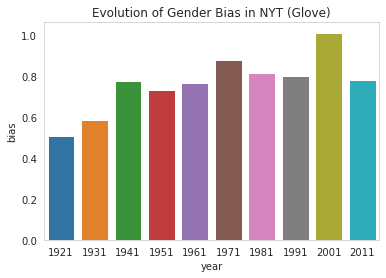
\includegraphics[width=0.45\linewidth]{images/glove_evolution.png}}
    \qquad
    \subfloat{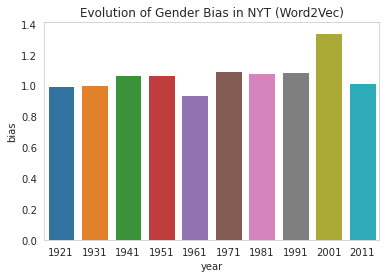
\includegraphics[width=0.45\linewidth]{images/word2vec_evolution.png}}
\caption{Evolution of bias in NYT 100 Years dataset}
    \label{fig:evolution}
\end{figure}

This ~\ref{fig:evolution} illustrates the progression of bias over time. To generate this plot, 100 years is first divided into 10 datasets, each corresponding to a decade. Then for each decade, a model is trained and then bias is calculated using WEAT. This is done for three different models, word2vec and glove.

In these plots y axis is the average bias score for each model, which is calculated on the basis of 7 WEAT tests. X axis is the decade of the model.

\subsection{Part 2: Bias manifold is linear}

\begin{figure}[H]
    \centering
    \subfloat{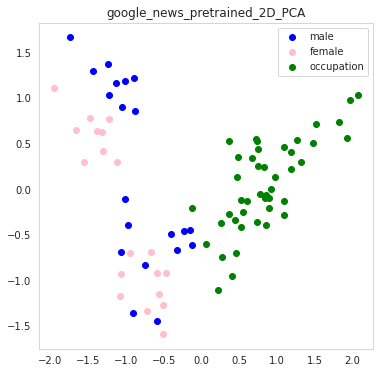
\includegraphics[width=0.45\linewidth]{images/google_news_2D_PCA.png}}
    \qquad
    \subfloat{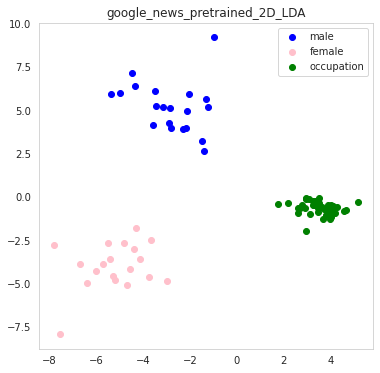
\includegraphics[width=0.45\linewidth]{images/google_news_2D_LDA.png}}
\caption{Dimensionality of Bias (Google News Word2Vec model)}
    \label{fig:bias_manifold_google_news}
\end{figure}


\begin{figure}[H]
    \centering
    \subfloat{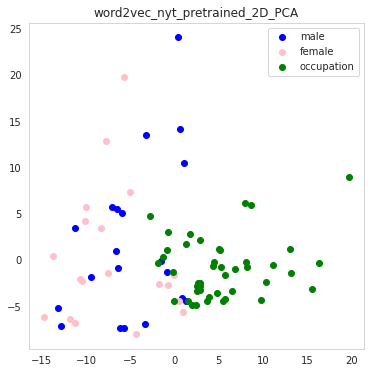
\includegraphics[width=0.45\linewidth]{images/word2vec_2D_PCA.png}}
    \qquad
    \subfloat{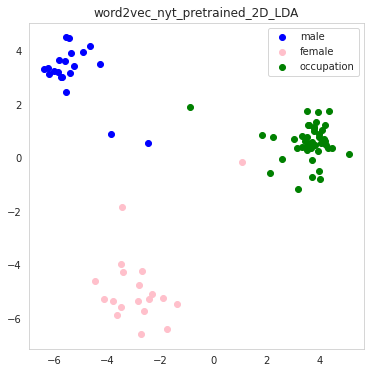
\includegraphics[width=0.45\linewidth]{images/word2vec_2D_LDA.png}}
\caption{Dimensionality of Bias (NYT Word2Vec model)}
    \label{fig:bias_manifold_word2vec}
\end{figure}


\begin{figure}[H]
    \centering
    \subfloat{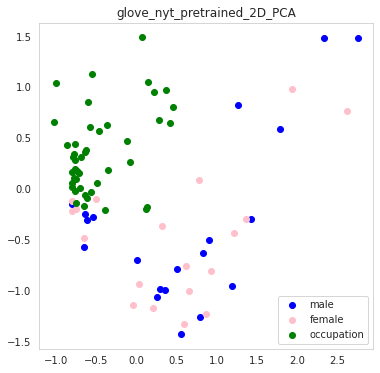
\includegraphics[width=0.45\linewidth]{images/glove_2D_PCA.png}}
    \qquad
    \subfloat{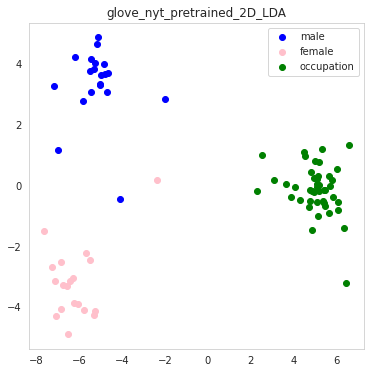
\includegraphics[width=0.45\linewidth]{images/glove_2D_LDA.png}}
\caption{Dimensionality of Bias (NYT Glove model)}
    \label{fig:bias_manifold_glove}
\end{figure}

In these plots I am trying to see if bias manifold is linear or not. To do this I am using two different methods, PCA and LDA. Blue points are male oriented, pink points are female oriented and green points are neutral occupation names, as demonstrated by legends in the plot. Models are google news word2vec model, and the last models each from word2vec and glove trained on NYT 2011-2021 dataset. Conclusions are drawn in the next section.

These plots are generated by first loading pretrained models in memory and then using them to predict embeddings of these words. Then PCA or LDA are used to project those in two dimensions. The notebook which generates these plots also plots 3 D images of the same. But I have not included them here because they are not very useful for our analysis here.

\subsection{Part 3: Most biased documents in a dataset}

\begin{figure}[H]
    \centering
    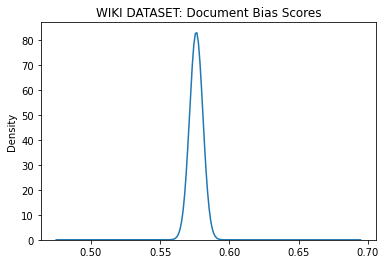
\includegraphics[width=\textwidth]{images/document_weat_scores.png}
    \caption{Distribution of Weat Scores after applying Bias Gradient per document}
    \label{fig:document_weat_scores}
\end{figure}

This plot shows the distribution of weat scores derived from applying bias gradient to the glove model for each document and evaluating those model weights on our WEAT evaluation set. This is a kde plot where x axis is the average weat score for each document and y axis is the density of documents with that score. This plot is generated by loading the scores generated by the driver file which is part of the github repository.

\section{Discussion}

\subsection{Interpretation of results}

Following sections reflect on the results and try to answer the questions posed in the beginning of the project. At times they also discuss the reason behind the results and why they may not be very dependable.

\subsubsection{Part 1: Bias manifold evolution over time}

Contrary to what I was expecting, bias seems to be either increasing or remaining more or less same in the plots ~\ref{fig:evolution}. My thinking was that over period of time people tend to become less and less biased and this is reflected in their writings.

But this is not the case. I think this is because of the fact that we are using a very small dataset to train our models or evaluate the model. This could be result of wrong assumptions as well.


\subsubsection{Part 2: Bias manifold is linear}

This was an interesting result to look. As expected \"gender bias\" is definitely linear. We demonstrate this with three different models, and two different sets. However one point to note here that PCA does not work very well in separating the different clusters, probably because it is not supervised method. LDA on the other hand does a good job of separating the clusters. This is because LDA is a supervised method and it uses the labels to separate the clusters.

Results are consistent across different models and we can see that three clusters in question here are linearly separable.


\subsubsection{Part 3: Most biased documents in a dataset}

As we can see in ~\ref{fig:document_weat_scores}, the distribution of weat scores is as expected. Most of the documents are neutral and there are very few documents which are very biased. In future work may this score can be used to identify the most biased documents in a dataset and then after removing those documents we can train a model which is less biased. This method in both horizontally and vertically scalable. Horizontally because we can add more test sets and then taking mean, vertical because we can increase the train dataset and both of these scalings will help to learn a better and fairer model.

\subsection{Skills from course that were used}

There are many skills that I have learned from this course that I have used in this project. For example different fairness paradigms, deep learning, and using jupyter lab through different assignments. Introduction to different fairness metrics and AI 360 was helpful in understanding the problem statement and how to approach it.

Other skills that were helpful were software architecture, systems design, data modelling, and data engineering.

\subsection{Failures and challenges}

 There were lot of challenges and failures, but I will try to list the most important ones here.
\begin{itemize}
    \item Was not able to complete bias evolution using Jackknife, because of the time it requires to train all models.
    \item WEAT evaluation dataset was very small. I tried searching for more datasets but could not find any. May be in one of future future projects I can try to create a dataset which is more representative of the population.
    \item This is more of future work, but I could've used bias gradient score to trim the dataset and then train a model which is less biased.
    \item Also in the project I only use gender bias to do my analysis. It would have been better if I could try different bias types and see how they evolve over time. Even in this case I would've required a WEAT evaluation dataset, which was not available.
\end{itemize}

\section{Conclusion}

I think this was very fruitful project. I learnt a lot about different bias metrics, fairness. I went through almost all the research I cited. This was a very enlightening experience. I hope to continue work in this same direction in future.


\begin{acks}
\end{acks}



\bibliographystyle{alpha}

\bibliography{base}

\end{document}
\endinput